% ==========================================================
\chapter{集合・写像・同値関係}\label{app:A}
% ==========================================================

この付録では，本編全体で断りなく用いる集合論の言葉をまとめる．
特に「同値関係で割って商集合を作る」という操作は，
剰余環 $R/I$（第2章），座標環 $k[X]=k[x_1,\dots,x_n]/\Ideal(X)$（第5章），
射影空間 $\PP^n=(k^{n+1}\setminus\{0\})/k^\times$（第8章），
モジュライ空間（第16章）など，本編のあらゆる場面に現れる．
最後の節では商集合の普遍性を述べ，「商は普遍性で特徴づけられる」という
本編で繰り返し使う考え方を準備する．

% ----------------------------------------------------------
\section{集合と部分集合}
% ----------------------------------------------------------

集合とは，ものの集まりであって，任意のもの $a$ について
「$a$ がその集合に属するか否か」が確定しているものをいう．
$a$ が集合 $X$ に属することを $a\in X$ と書き，$a$ を $X$ の\textbf{元}（要素）という．

\begin{mydef}{部分集合}{appA-subset}
集合 $X,Y$ について，$X$ の任意の元が $Y$ の元であるとき，$X$ は $Y$ の\textbf{部分集合}であるといい，
$X\subset Y$ と書く．$X\subset Y$ かつ $Y\subset X$ のとき $X=Y$ である．
元を一つも持たない集合を\textbf{空集合}といい $\emptyset$ と書く．
\end{mydef}

本ノートでは $\subset$ は等号を許す包含を表す．真の包含を強調するときは $\subsetneq$ と書く．

集合 $X$ の部分集合 $A,B$ に対して
\[
A\cup B=\{x\mid x\in A \text{ または } x\in B\},\quad
A\cap B=\{x\mid x\in A \text{ かつ } x\in B\},
\]
\[
A\setminus B=\{x\in A\mid x\notin B\},\qquad A^c=X\setminus A
\]
をそれぞれ\textbf{和集合}，\textbf{共通部分}，\textbf{差集合}，\textbf{補集合}という．
添字集合 $\Lambda$ で添字づけられた部分集合の族 $\{A_\lambda\}_{\lambda\in\Lambda}$ に対しても
$\bigcup_{\lambda}A_\lambda$，$\bigcap_\lambda A_\lambda$ が同様に定義される．

\begin{myprop}{de Morgan の法則}{appA-demorgan}
集合 $X$ の部分集合の族 $\{A_\lambda\}_{\lambda\in\Lambda}$ に対して
\[
\Bigl(\bigcup_{\lambda\in\Lambda}A_\lambda\Bigr)^c=\bigcap_{\lambda\in\Lambda}A_\lambda^c,\qquad
\Bigl(\bigcap_{\lambda\in\Lambda}A_\lambda\Bigr)^c=\bigcup_{\lambda\in\Lambda}A_\lambda^c .
\]
\end{myprop}
\begin{proof}
$x\notin\bigcup A_\lambda$ $\iff$ すべての $\lambda$ で $x\notin A_\lambda$ $\iff$ $x\in\bigcap A_\lambda^c$．
後半も同様である．
\end{proof}

この法則により，「閉集合の公理」と「開集合の公理」は補集合をとることで互いに移り合う．
第3章で Zariski 位相を閉集合（代数的集合）の側から定義するのはこの事実による．

\begin{mydef}{冪集合}{appA-powerset}
集合 $X$ の部分集合全体のなす集合を $X$ の\textbf{冪集合}といい，$2^X$ または $\mathcal{P}(X)$ と書く．
\end{mydef}

\begin{myex}{零点集合と消滅イデアル}{appA-VI}
$k$ を体とし $R=k[x_1,\dots,x_n]$ とする．多項式の部分集合 $S\subset R$ に対して
$\Zero(S)=\{a\in k^n\mid f(a)=0\ (\forall f\in S)\}$ と置くと，
$\Zero$ は写像 $2^R\to 2^{k^n}$ である．逆向きに $X\subset k^n$ に対して
$\Ideal(X)=\{f\in R\mid f(a)=0\ (\forall a\in X)\}$ と置けば $\Ideal\colon 2^{k^n}\to 2^R$ を得る．
どちらも包含関係を逆転する：$S\subset T\Rightarrow \Zero(S)\supset\Zero(T)$．
この「包含の逆転」が第4章の代数と幾何の対応の出発点である．
\end{myex}

% ----------------------------------------------------------
\section{直積集合}
% ----------------------------------------------------------

\begin{mydef}{直積}{appA-product}
集合 $X,Y$ の\textbf{直積}を
\[
X\times Y=\{(x,y)\mid x\in X,\ y\in Y\}
\]
で定める．$(x,y)=(x',y')$ は $x=x'$ かつ $y=y'$ を意味する．
$n$ 個の集合の直積 $X_1\times\dots\times X_n$ も同様に定義し，$X\times\dots\times X$（$n$ 個）を $X^n$ と書く．
\end{mydef}

射影 $\pi_1\colon X\times Y\to X$，$(x,y)\mapsto x$ および $\pi_2\colon X\times Y\to Y$ を
\textbf{標準射影}という．直積は次の普遍性で特徴づけられる：
任意の集合 $Z$ と写像 $f\colon Z\to X$，$g\colon Z\to Y$ に対して，
$\pi_1\circ h=f$，$\pi_2\circ h=g$ を満たす写像 $h\colon Z\to X\times Y$ が
ただ一つ存在する（$h(z)=(f(z),g(z))$）．
\[
\begin{tikzcd}
 & Z \arrow[ld,"f"'] \arrow[d,dashed,"h"] \arrow[rd,"g"] & \\
X & X\times Y \arrow[l,"\pi_1"] \arrow[r,"\pi_2"'] & Y
\end{tikzcd}
\]

\begin{myex}{アフィン空間}{appA-affine}
体 $k$ に対し $k^n=k\times\dots\times k$ は $n$ 個の $k$ の直積である．
第3章のアフィン空間 $\A^n$ は集合としては $k^n$ であり，その上に Zariski 位相を入れたものである．
ただし $\A^m\times\A^n=\A^{m+n}$ 上の Zariski 位相は，$\A^m$ と $\A^n$ の Zariski 位相の積位相
（付録E）とは一致しない（積位相より真に細かい）ことに注意する．
\end{myex}

\begin{mydef}{関係}{appA-relation}
集合 $X$ 上の\textbf{二項関係}とは，直積 $X\times X$ の部分集合 $R$ のことである．
$(x,y)\in R$ のとき $x\,R\,y$ あるいは $x\sim y$ と書く．
\end{mydef}

% ----------------------------------------------------------
\section{写像}
% ----------------------------------------------------------

\begin{mydef}{写像}{appA-map}
集合 $X,Y$ に対し，$X$ の各元 $x$ に $Y$ の元 $f(x)$ をただ一つ対応させる規則を
$X$ から $Y$ への\textbf{写像}といい，$f\colon X\to Y$ と書く．$X$ を\textbf{定義域}，$Y$ を\textbf{終域}という．
厳密には，写像とは部分集合 $\Gamma_f\subset X\times Y$（\textbf{グラフ}）であって，
各 $x\in X$ に対して $(x,y)\in\Gamma_f$ となる $y$ がただ一つ存在するもののことである．
\end{mydef}

写像 $f\colon X\to Y$ と部分集合 $A\subset X$，$B\subset Y$ に対して
\[
f(A)=\{f(a)\mid a\in A\}\ (\text{像}),\qquad
f^{-1}(B)=\{x\in X\mid f(x)\in B\}\ (\text{逆像})
\]
と定める．逆像は和・共通部分・補集合と可換である：
\[
f^{-1}\Bigl(\bigcup B_\lambda\Bigr)=\bigcup f^{-1}(B_\lambda),\quad
f^{-1}\Bigl(\bigcap B_\lambda\Bigr)=\bigcap f^{-1}(B_\lambda),\quad
f^{-1}(B^c)=f^{-1}(B)^c .
\]
一方，像は一般に共通部分とは可換でない（$f(A\cap A')\subsetneq f(A)\cap f(A')$ となりうる）．
連続写像を「開集合の逆像が開」で定義する（付録E）のは，逆像のこの良い性質による．

\begin{mydef}{合成・恒等写像・制限}{appA-comp}
$f\colon X\to Y$，$g\colon Y\to Z$ に対し，$(g\circ f)(x)=g(f(x))$ で定まる写像
$g\circ f\colon X\to Z$ を\textbf{合成}という．合成は結合的である：$h\circ(g\circ f)=(h\circ g)\circ f$．
$\mathrm{id}_X(x)=x$ を\textbf{恒等写像}という．
$A\subset X$ に対し，$f$ を $A$ 上でのみ考えた写像を\textbf{制限}といい $f|_A$ と書く．
\end{mydef}

\begin{myex}{多項式写像の引き戻し}{appA-pullback}
写像 $\varphi\colon X\to Y$ と $Y$ 上の関数 $g\colon Y\to k$ があると，
合成 $g\circ\varphi\colon X\to k$ は $X$ 上の関数になる．これを $\varphi^*g$ と書き，\textbf{引き戻し}という．
$\varphi^*(g_1g_2)=\varphi^*g_1\cdot\varphi^*g_2$，$\varphi^*(g_1+g_2)=\varphi^*g_1+\varphi^*g_2$ が成り立ち，
また $(\psi\circ\varphi)^*=\varphi^*\circ\psi^*$ と順序が逆転する．
第5章では，この $\varphi^*$ が座標環の間の環準同型 $k[Y]\to k[X]$ を与えることを見る（反変性）．
\end{myex}

集合 $X$ から $Y$ への写像全体の集合を $\mathrm{Map}(X,Y)$ あるいは $Y^X$ と書く．
添字集合 $\Lambda$ からの写像 $\lambda\mapsto x_\lambda$ を\textbf{族} $(x_\lambda)_{\lambda\in\Lambda}$ ということがある．

% ----------------------------------------------------------
\section{単射・全射・全単射}
% ----------------------------------------------------------

\begin{mydef}{単射・全射・全単射}{appA-inj}
写像 $f\colon X\to Y$ について
\begin{itemize}
\item $f(x)=f(x')\Rightarrow x=x'$ が成り立つとき\textbf{単射}という．
\item $f(X)=Y$ のとき\textbf{全射}という．
\item 単射かつ全射のとき\textbf{全単射}という．
\end{itemize}
\end{mydef}

\begin{myprop}{逆写像}{appA-inverse}
$f\colon X\to Y$ が全単射であることと，$g\circ f=\mathrm{id}_X$ かつ $f\circ g=\mathrm{id}_Y$ を満たす
$g\colon Y\to X$ が存在することは同値である．このとき $g$ は一意的であり，$f$ の\textbf{逆写像} $f^{-1}$ という．
\end{myprop}
\begin{proof}
$f$ が全単射なら，各 $y\in Y$ に対して $f(x)=y$ となる $x$ がただ一つあるので $g(y)=x$ と置けばよい．
逆に $g$ があれば，$f(x)=f(x')$ から $x=g(f(x))=g(f(x'))=x'$ で単射，
$y=f(g(y))$ から全射．一意性は $g=g\circ(f\circ g')=(g\circ f)\circ g'=g'$ による．
\end{proof}

より一般に，$X\ne\emptyset$ のとき，$f$ が単射 $\iff$ 左逆写像 $g$（$g\circ f=\mathrm{id}_X$）が存在する．
また $f$ が全射 $\iff$ 右逆写像 $s$（$f\circ s=\mathrm{id}_Y$）が存在する（後者は選択公理を用いる）．
全射の右逆写像 $s$ を\textbf{切断}（section）とよぶ．
この言葉は，ベクトル束 $\pi\colon E\to M$ の切断 $s\colon M\to E$，$\pi\circ s=\mathrm{id}_M$（付録F，第14章）
の語源でもある．

\begin{myex}{}{appA-injex}
\begin{enumerate}
\item 包含写像 $\iota\colon A\hookrightarrow X$ は単射である．
\item 標準射影 $\pi_1\colon X\times Y\to X$ は（$Y\ne\emptyset$ なら）全射である．
\item $\C\to\C$，$z\mapsto z^2$ は全射だが単射でない．$\R\to\R$，$x\mapsto x^2$ は全射でも単射でもない．
代数閉体上では方程式が常に解を持つという性質が，第1章で複素数上の代数幾何を考える理由の一つである．
\item 多項式写像 $\A^1\to\Zero(y^2-x^3)\subset\A^2$，$t\mapsto(t^2,t^3)$ は全単射であるが，
逆写像は多項式写像にならない（第5章・第7章のカスプの例）．
\end{enumerate}
\end{myex}

\begin{note}
集合の間の全単射は「集合として同じ」ことを意味するにすぎない．
代数幾何では，構造（位相・関数の層）を保つ同型の方がはるかに重要であり，
上の (4) のように全単射であっても同型でない射がしばしば現れる．
\end{note}

% ----------------------------------------------------------
\section{同値関係}
% ----------------------------------------------------------

\begin{mydef}{同値関係}{appA-equiv}
集合 $X$ 上の二項関係 $\sim$ が次の3条件を満たすとき\textbf{同値関係}という．
\begin{enumerate}
\item（反射律）すべての $x\in X$ について $x\sim x$．
\item（対称律）$x\sim y\Rightarrow y\sim x$．
\item（推移律）$x\sim y$ かつ $y\sim z\Rightarrow x\sim z$．
\end{enumerate}
\end{mydef}

\begin{mydef}{同値類}{appA-class}
同値関係 $\sim$ と $x\in X$ に対して
\[
[x]=\{y\in X\mid y\sim x\}
\]
を $x$ の\textbf{同値類}という．$[x]$ の元を同値類の\textbf{代表元}という．
\end{mydef}

\begin{myprop}{同値類による分割}{appA-partition}
$\sim$ を $X$ 上の同値関係とする．
\begin{enumerate}
\item $x\sim y\iff [x]=[y]$．
\item $[x]\cap[y]\ne\emptyset$ ならば $[x]=[y]$．
\item $X$ は相異なる同値類の互いに素な和集合である．
\end{enumerate}
逆に，$X$ の互いに素な空でない部分集合への分割が与えられれば，
「同じ部分集合に属する」という関係は同値関係である．
\end{myprop}
\begin{proof}
(1) $x\sim y$ とし $z\in[x]$ とすると $z\sim x\sim y$ より $z\in[y]$．対称律より逆の包含も従う．
逆に $[x]=[y]$ なら $x\in[x]=[y]$ より $x\sim y$．
(2) $z\in[x]\cap[y]$ なら $x\sim z\sim y$ で (1) より $[x]=[y]$．
(3) 反射律より $x\in[x]$ なので各元はいずれかの同値類に属し，(2) より相異なる同値類は交わらない．
\end{proof}

\begin{myex}{基本的な同値関係}{appA-equivex}
\begin{enumerate}
\item 整数 $n\geq1$ に対し，$\Z$ 上で $a\sim b\iff n\mid(a-b)$ は同値関係である（合同）．
\item 環 $R$ とイデアル $I$ に対し，$a\sim b\iff a-b\in I$ は同値関係である（第2章，剰余環）．
\item $k^{n+1}\setminus\{0\}$ 上で $x\sim y\iff$ ある $\lambda\in k^\times$ で $y=\lambda x$，は同値関係である（第8章，射影空間）．
重み $(w_0,\dots,w_n)$ を付けて $y=(\lambda^{w_0}x_0,\dots,\lambda^{w_n}x_n)$ とすれば重み付き射影空間（第15章）を得る．
\item 群 $G$ が集合 $X$ に作用しているとき，$x\sim y\iff$ ある $g\in G$ で $y=g\cdot x$，は同値関係である．
同値類は\textbf{軌道}である．ゲージ変換で移り合う場の配位を同一視する操作はこの形をしている（第14章，第16章）．
\item 多様体の同型「$X\cong Y$」は（集合論的な注意を除けば）同値関係であり，
その同値類の全体を幾何学的に記述しようとするのがモジュライ問題（第16章）である．
\end{enumerate}
\end{myex}

\begin{note}
「関係 $\sim$ を生成する同値関係」とは，$\sim$ を含む最小の同値関係，すなわち
$\sim$ を含むすべての同値関係（$X\times X$ の部分集合）の共通部分のことである．
貼り合わせ（第8章のチャート，第12章のスキーム）では，貼り合わせ写像で定まる関係から生成される同値関係で割る．
\end{note}

% ----------------------------------------------------------
\section{商集合}
% ----------------------------------------------------------

\begin{mydef}{商集合}{appA-quotient}
集合 $X$ 上の同値関係 $\sim$ に対し，同値類全体の集合
\[
X/{\sim}=\{[x]\mid x\in X\}
\]
を\textbf{商集合}という．写像 $\pi\colon X\to X/{\sim}$，$x\mapsto[x]$ を\textbf{標準射影}（自然な射影）という．
$\pi$ は全射である．
\end{mydef}

\begin{myex}{}{appA-quotex}
\begin{enumerate}
\item 合同関係による商集合 $\Z/n\Z=\{[0],[1],\dots,[n-1]\}$．
\item 環 $R$ のイデアル $I$ による商集合 $R/I=\{a+I\mid a\in R\}$．
同値類 $[a]$ は剰余類 $a+I$ そのものである．
\item $\PP^n=(k^{n+1}\setminus\{0\})/{\sim}$．点 $[x_0:\dots:x_n]$ は原点を通る直線 $\{\lambda x\}$ に対応する．
\item 実数直線 $\R$ を $x\sim y\iff x-y\in\Z$ で割ると円周 $\R/\Z\cong S^1$ を得る．
同様に $\C/(\Z+\tau\Z)$（$\operatorname{Im}\tau>0$）は複素トーラス，すなわち楕円曲線である（第13章，第17章）．
\end{enumerate}
\end{myex}

\begin{figure}[H]
\centering
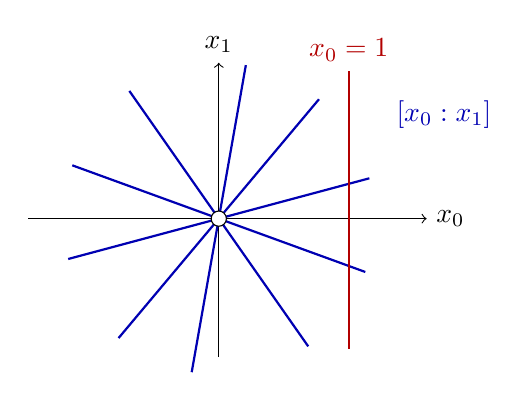
\begin{tikzpicture}[scale=1.1]
  \draw[->] (-2.2,0)--(2.4,0) node[right]{$x_0$};
  \draw[->] (0,-1.6)--(0,1.8) node[above]{$x_1$};
  \foreach \a in {15,50,80,125,160} {
    \draw[thick,blue!70!black] ({-1.8*cos(\a)},{-1.8*sin(\a)}) -- ({1.8*cos(\a)},{1.8*sin(\a)});
  }
  \fill[white] (0,0) circle (2.5pt); \draw (0,0) circle (2.5pt);
  \node[blue!70!black] at (2.6,1.2) {$[x_0:x_1]$};
  \draw[red!70!black,thick] (1.5,-1.5)--(1.5,1.7) node[above]{$x_0=1$};
\end{tikzpicture}
\caption{$\PP^1$ の点は $k^2\setminus\{0\}$ の原点を通る直線（同値類）である．
直線 $x_0=1$ と交わる同値類は代表元 $(1,x_1/x_0)$ を一意に持つ（アフィンチャート，第8章）．}
\end{figure}

\begin{myprop}{代表元によるwell-definedness}{appA-welldef}
写像 $f\colon X\to Y$ が「$x\sim x'\Rightarrow f(x)=f(x')$」を満たすとき，
$\bar f([x])=f(x)$ によって写像 $\bar f\colon X/{\sim}\to Y$ が矛盾なく（well-defined に）定まる．
\end{myprop}
\begin{proof}
$[x]=[x']$ なら $x\sim x'$ なので $f(x)=f(x')$ であり，$\bar f([x])$ の値は代表元の取り方によらない．
\end{proof}

このように，商集合上の写像や演算を代表元を用いて定義するときは，
代表元の選び方によらないこと（well-definedness）を必ず確認しなければならない．
たとえば剰余環 $R/I$ の積 $(a+I)(b+I)=ab+I$ が well-defined であるのは，
$I$ が\emph{イデアル}であって単なる部分加群でないからである（第2章）．

\begin{myex}{射影空間上では多項式の値は定まらない}{appA-homog}
$f\in k[x_0,\dots,x_n]$ に対し $[x]\mapsto f(x)$ は一般に well-defined でない．
しかし $f$ が $d$ 次同次多項式なら $f(\lambda x)=\lambda^d f(x)$ なので，
「$f(x)=0$ か否か」は代表元によらない．したがって同次多項式の零点集合は $\PP^n$ の部分集合として意味を持つ（第8章）．
また同じ次数の同次多項式の比 $f/g$ は $\{g\ne0\}$ 上で well-defined な関数になる．
\end{myex}

% ----------------------------------------------------------
\section{商集合の普遍的な考え方}
% ----------------------------------------------------------

前節の命題は，次の\textbf{普遍性}としてまとめられる．

\begin{mythm}{商集合の普遍性}{appA-univ}
$\sim$ を $X$ 上の同値関係，$\pi\colon X\to X/{\sim}$ を標準射影とする．
写像 $f\colon X\to Y$ が「$x\sim x'\Rightarrow f(x)=f(x')$」を満たすならば，
$f=\bar f\circ\pi$ を満たす写像 $\bar f\colon X/{\sim}\to Y$ がただ一つ存在する．
\[
\begin{tikzcd}
X \arrow[r,"f"] \arrow[d,"\pi"'] & Y\\
X/{\sim} \arrow[ru,dashed,"\exists!\,\bar f"'] &
\end{tikzcd}
\]
\end{mythm}
\begin{proof}
存在は命題\ref{prop:appA-welldef}による．一意性：$\bar f\circ\pi=\bar f'\circ\pi$ であり $\pi$ は全射なので $\bar f=\bar f'$．
\end{proof}

逆に，この普遍性は商集合を「同型を除いて一意に」特徴づける．

\begin{myprop}{普遍性による一意性}{appA-unique}
集合 $Q$ と写像 $q\colon X\to Q$ が，$x\sim x'\Rightarrow q(x)=q(x')$ を満たし，
かつ定理\ref{thm:appA-univ}と同じ普遍性（$\pi$ を $q$ に置き換えたもの）を持つとする．
このとき $\bar q\colon X/{\sim}\to Q$ は全単射で，$\bar q\circ\pi=q$ を満たす．
\end{myprop}
\begin{proof}
$\pi$ の普遍性から $\bar q\colon X/{\sim}\to Q$ が，$q$ の普遍性から $\bar\pi\colon Q\to X/{\sim}$ が得られる．
$\bar\pi\circ\bar q\circ\pi=\bar\pi\circ q=\pi=\mathrm{id}\circ\pi$ であり，$\pi$ の普遍性の一意性部分から
$\bar\pi\circ\bar q=\mathrm{id}$．同様に $\bar q\circ\bar\pi=\mathrm{id}$．
\end{proof}

この「普遍性 $\Rightarrow$ 同型を除いて一意」という議論は，本編で何度も現れる．
\begin{itemize}
\item 剰余環 $R/I$ の普遍性（第2章）：$\Ker\varphi\supset I$ なる環準同型 $\varphi\colon R\to S$ は
$\bar\varphi\colon R/I\to S$ を一意に誘導する．準同型定理 $R/\Ker\varphi\cong\Img\varphi$ はこの特別な場合である．
\item 局所化 $S^{-1}R$ の普遍性（第6章）．
\item 商位相（付録E）：商集合に，標準射影が連続になる最も細かい位相を入れたもの．
\item 圏論における余極限（付録G）．
\end{itemize}

\begin{myex}{全射による商}{appA-surj}
任意の写像 $f\colon X\to Y$ は，$x\sim x'\iff f(x)=f(x')$ で同値関係を定める．
このとき $\bar f\colon X/{\sim}\to f(X)$ は全単射であり，
\[
X\xrightarrow{\ \pi\ }X/{\sim}\xrightarrow{\ \bar f\ }f(X)\xrightarrow{\ \iota\ }Y
\]
と分解する（全射・全単射・単射への分解）．群・環・ベクトル空間の準同型定理は，
これに演算との整合性を付け加えたものである（付録B，付録C）．
\end{myex}

\begin{physbox}[商としての物理的状態空間]
物理では「同じ物理状態を表す記述」を同一視することが基本的な操作である．
量子力学の状態はヒルベルト空間のベクトル $\psi\ne0$ を $\psi\sim\lambda\psi$（$\lambda\in\C^\times$）で割った
射影空間の点であり，ゲージ理論の物理的配位はゲージ場の空間をゲージ変換群の作用で割った軌道空間である．
商集合にどのような位相・幾何構造が入るか（Hausdorff か，特異点を持つか）は一般には微妙な問題であり，
第16章のモジュライ空間の議論でこの問題に再び出会う．
\end{physbox}
